% Trust
% TPRC 2016 Submission
%
% Spring 2016
%
% Andy Sayler

\documentclass[11pt,letterpaper]{article}

% System Packages
\usepackage[margin=1in]{geometry}
\usepackage{epsfig}
\usepackage{float}
\usepackage[dvipsnames]{xcolor}
\usepackage{caption}
\usepackage{subcaption}
\usepackage{tabu}
\usepackage{hyperref}
\usepackage{url}
\usepackage[affil-it]{authblk}

% Local Packages
% None

% Package Options
\hypersetup{
    colorlinks,
    citecolor=black,
    filecolor=black,
    linkcolor=black,
    urlcolor=black
}

% Macros
\input{macros.tex}

% Other Options
\clubpenalty = 10000
\widowpenalty = 10000

% Start
\begin{document}

\title{Categorizing, Analyzing, and Managing Third Party Trust}

\author{Andy Sayler}
\affil{University of Colorado, Boulder}

\date{}

\maketitle

\begin{abstract}

The modern computing ecosystem requires users to trust a variety of
third parties to complete even the most basic of digital tasks.  From
system administers to service providers to device manufactures, which
third parties computer users must trust and the capabilities with
which they must trust them is a critical component underpinning the
privacy and security of our digital data. The rise of the ``cloud'' as
the preferred platform for most modern computing applications makes
questions of trust even more complicated and pressing. A lack of
understanding or misplacement of such trust has the potential to lead
to data leaks, questionable surveillance practices, and a wide range
of related privacy-harming events.

It is thus desirable from a public policy perspective to help
individuals understand and control third party trust and to minimize
the likelihood of such trust being violated. Toward these ends, this
paper presents a model for describing third party trust and the
likelihood of trust violations. It applies this model to analyze the
nature of third party trust across of a variety of popular cloud
services and uses it to categorize the common manners in which third
parties violate this trust. Finally, this paper presents a number of
proposed techniques, both technological and policy-based, to minimize
the degree of trust users must place in third parties as well as to
decrease the likelihood of violation of this trust.

\end{abstract}

\section{Introduction}
\label{sec:intro}

Trust and privacy are closely related qualities in computing. Can
users maintain their digital privacy without having to trust anyone?
One can imagine scenarios that maintain privacy without trust, but
such scenarios generally involve only storing data on self-designed,
built, and programmed devices that never leave one's possession. Such
an arrangement is, at best, impractical for the vast majority of
users, and at worst, simply not possible to achieve today. The range
of manufactures, developers, and service providers inherent in the
modern computing landscape require that users make decisions regarding
whom to trust at every step of any digital interaction in which they
partake.

The cloud computing model, by its very nature, further amplifies the
number of parties users must trust. Individuals regularly place their
trust in third parties such as Facebook, Dropbox, Google, and
countless others to securely store their files, relay their
communications, or process their data. But is this trust well placed?
A range of recent data breaches effecting entities ranging from health
insurance providers to the U.S. Government can be traced back to
violations of the trust that users place in third parties. This fact
raises a number of additional questions. With which capabilities are
users required to trust third parties? In what manners can this trust
be violated? Is this trust an implicit necessity, or are there ways to
reduce the trust users must place in third parties. And finally, are
there policy mechanisms that can be used to reduce the likelihood of
third party trust violations.

This paper aims to discuss and provide answers to these questions.

\subsection{Background}

Trust has long been a key component of computing
security~\cite{thompson1984}.

\section{Modeling Trust}
\label{sec:model}

Researchers from a variety of disciplines have proposed a range of
trust definitions and models~\cite{camp2003, flowerday2006,
  grandison2000, sabater2005}. These models range from technical
models for calculating reputations via machine-learning algorithms to
sociological models for exploring legal and societal notions of
trust. In this section, I propose a trust model for exploring the
manner in which users interact with third parties across the modern
computing landscape. In particular, this model aims to provide a basis
for describing how users trust third parties with access to their
digital data and the manners in which this trust might be violated.

Before defining a model for trust, it is useful to define some of the
relevant terms used in this model. To start, I'll define
\textit{trust} as the expectation that a given entity will behave in a
promised manner. \textit{Violations} of trust thus occur whenever said
entity deviates from this expectation. Trust is closely related to two
other properties inherent in modern computing ecosystems: security and
privacy. Like trust, these terms have wide-ranging meanings across a
variety of disciplines. For the purposes of this discussion, I'll
define \textit{security} as the notion of user control over the
behavior of a given system. A \textit{secure system} is thus a system
that behaves in the manner the user desires. Facets of this notion of
security include \textit{confidentiality}, the ability to control who
can read user data, and \textit{authenticity}, the ability to control
who can modify user data. Finally, confidentiality and authenticity
provide a definition of \textit{privacy} as the ability to control
both the access and modification of user data as well as the ability
to control the meta-record of such access or modification.

When users leverage modern computing devices and services, they must
trust third party manufacturers and service providers to be good
stewards of digital data ranging from stored files to location
information to communication messages. The nature of this trust has
two main factors:

\begin{packed_desc}
\item[Degree:] How much trust must a user place in a third party
  (e.g., what capabilities do they allow a third party to exercise
  with respect to user data)?
\item[Violation:] In what manners can the third party violate this
  trust (e.g., how can the third party abuse the capabilities they
  have been granted or why might they be inclined to do so)?
\end{packed_desc}

The security and privacy of a user's data is generally dependent on
these two axes: the higher the degree of trust a user places in a
third party, the more power that party has to subvert the privacy or
security of a user's data. Similarly, the higher the risk of third
party trust violations, the higher the risk of adverse effects to
security or privacy.  Intuitively, the best ways to enhance the
security and privacy of user data is thus to minimize degree of third
party trust, to minimize the likelihood of third party trust
violations, or to minimize both.

\subsection{Degree of Trust}

Degrees of trust measure the capabilities a third party can exert over
user data. I propose that third parties can be trusted with the
following data-related capabilities:

\begin{packed_desc}
\item[Storage (S-Capability):] \hfill \\ Can a third party faithfully
  store user data and make it available to the user upon request?
  Misuse of this capability may result in a loss of user data, but
  won't necessarily result in the exposure of user data.
\item[Access (R-Capability):] \hfill \\ Can a third party read and
  interpret the user data they store? Misuse of this capability may
  result in the unapproved exposure of user data.
\item[Manipulation (W-Capability):] \hfill \\ Can a third party modify
  the private user data to which they have access? Misuse of this
  capability may result in the ability to manipulate a user
  (e.g., changing appointments on a user's calendar, etc).
\item[Meta-analysis (M-Capability):] \hfill \\ Can a third party
  gather metadata related to any user data or a user's behavior
  interacting with this data? Misuse of this capability may result in
  the ability to infer information about a user (e.g., a user's
  friends).
\end{packed_desc}

While there are likely additional capabilities users can entrust to
third parties, this collection represents the core set of data-related
capabilities most commonly entrusted to cloud service providers.

\subsection{Trust Violations}

Trust violation occurs when a third party exercises any of the above
capabilities without explicit user knowledge and consent. Put another
way, a trust violation occurs whenever a third party leverages a
capability with which they are entrusted in a manner in which the user
does not expect the capability to be leveraged. I propose classifying
such violations into four high-level categories. Each category is
defined by the manner in which the violation occurs and the
motivations behind it:

\begin{packed_desc}
\item[Implicit (P-Violation):] \hfill \\ This class of trust violation
  occurs when a third party violates a user's trust in a manner
  approved by the third party. An example might be sharing user data
  with a business partner (e.g. an advertiser). Often these violations
  aren't really ``violations'' since a user may have clicked through a
  Terms of Service agreement that ``granted'' permission for such use,
  but if the third party is willfully engaging in behavior that the
  user would not generally expect, an implicit trust violation has
  occurred.
\item[Compelled (C-Violation):] \hfill \\ This class of trust
  violation occurs when a third party is compelled by another actor to
  violate a user's trust. The most common example would be a third
  party being forced to turn over user data or records in response to
  a request from the government with jurisdiction over the party.
\item[Unintentional (U-Violation):] \hfill \\ This form of violation
  occurs when a third party unintentionally discloses or manipulates
  user data. An example would be a coding error that allows unfettered
  access to user data. Traditional ``hacking'' attacks also fall into
  this class insofar that such attacks are often possible due to
  unintentional flaws in the design of a ``secure'' system.
\item[Colluding (L-Violation):] \hfill \\ This class of violation
  occurs when multiple third parties collude to gain capabilities over
  user data beyond what the user intended each to have
  individually. An example of such a violation might occur if a user
  has granted two separate parties access to different portions of
  user data (e.g., location data stored with their cellular service
  provider and credit card transaction data stored with their bank)
  that could be combined to reveal more about the user than the user
  intended either party to know.
\end{packed_desc}

While this list of violation categories is far from exhaustive, it
does provide a good high-level framework for exploring the patterns
underlying trust violations and potential methods of mitigation.

\section{Analysis of Services}
\label{sec:analysis}

The trust model proposed in \S~\ref{sec:model} is primarily useful for
what it can tell us about the nature of user trust and the modern
computing landscape. As such, I apply the model to analyze the
capabilities granted to a number of popular third party computing
services.

\subsection{Third Party Capabilities}
\label{sec:analysis:capabilites}

Third party based ``cloud'' computing services have become extremely
popular over the previous 10 years.  The question of how
\textit{trustworthy} these services are is addressed later in
~\S~\ref{sec:analysis:violations}. In this section, I explore how
\textit{trusted} such service are. That is, how much trust must users
place in such services? The capability axis of my proposed model is
useful to quantify this trust.

\subsubsection{File Storage}

Cloud file storage is a popular third party use case. Services such as
Dropbox~\cite{dropbox}, Google Drive~\cite{google-drive}, and
Microsoft OneDrive~\cite{microsoft-onedrive} all provide users with
mechanisms for storing their files in the cloud, often for the purpose
of keeping files synced across multiple devices or to provide the
ability to share files or collaboratively edit them with other
users. Traditional cloud storage services such as Dropbox, Drive, and
OneDrive are similar enough in their operation that I will use Dropbox
as a stand in for the analysis of all three.

What capabilities is a normal Dropbox user entrusting to Dropbox?
Clearly, users must trust Dropbox to faithfully store their data since
that is Dropbox's core purpose. Users therefore grant Dropbox the
\emph{S} capability. Furthermore, users must also grant Dropbox the
ability to read and access their data (i.e. the \emph{R} capability)
in order to support Dropbox's sharing and syncing features. While
Dropbox doesn't generally utilize it, users are also effectively
granting Dropbox the manipulation (\emph{W} capability) as well since
the user has no mechanisms for ensuring that Dropbox can't manipulate
their data. Finally, Dropbox has full access to user metadata related
to their usage of the service, granting them the \emph{M}
capability. Therefore, Dropbox users must trust Dropbox with all
possible capabilities. Traditional cloud storage services such as
Dropbox, Drive, and OneDrive are thus classified as ``fully trusted''
services: service that require the highest possible level of user
trust. Such services, are thus also in a position to do the greatest
degree of damage to user privacy should a users trust in them as
faithful stewards of private data turn out to be misplaced.

The level of trust requested by tradition cloud storage servers
rightfully makes some user nervous or unwilling to use such
services. In response to such aversion, a number of systems have been
developed with the aim of overcoming third party trust challenges in
the storage space. These systems include ``end-to-end'' encrypted file
storage services such as Tresorit~\cite{tresorit}, or
SpiderOak~\cite{spideroak}. These systems aim to place limits on a
third party's ability to leverage the access (\emph{R}) capability
through the use of client-side encryption. Likewise, they aim to limit
third party access to the manipulation (\emph{W}) capability through
the use of client-side cryptographic
authentication.\footnote{E.g. asymmetric cryptographic signatures such
  as those provided by GnuPG~\cite{gnupg} or symmetric cryptographic
  message authentication codes (MACs) available via a variety of
  algorithms~\cite{dworkin2005, dworkin2007, dworkin2008}.}  In the
base case where a user merely wishes to store data on a single device
and not share it with others, these systems are fairly successful in
achieving their desired trust mitigations. In order to sync data
across multiple devices using such systems, a user must manually
provide some secret (e.g. a password, etc) on each device to secure
its operation. While potentially burdensome and inconvenient, this
practice is in line with these services trusted capabilities
mitigation since it does not require any additional third party trust.

The place where these systems falter at mitigating third party trust
is via their support for multi-user sharing and collaboration. Such
services tend to accomplish multi-user sharing by acting as a trusted
certificate authority (CA) in charge of issuing user
certificates.\footnote{A certificate is a combination of a user's
  public key and certain metadata signed by a trusted issuer. See for
  more information.}These certificates are then used with various
asymmetric cryptographic primitives) to exchange the necessary secrets
for bootstrapping sharing between users. Unfortunately, as a trusted
CA, these services are capable of issuing fraudulent user certificates
to themselves or other parties. This allows them to mount
man-in-the-middle (MitM) attacks on any user trying to share data by
impersonating the recipient of the shared data. This deficiency is
discussed in depth at~\cite{wilson2014}, and leads to a breakdown of
such services' claim that their users need not trust them, at least
when employing multi-user sharing. By mounting a MitM attack on a user
trying to share data with another user, such service providers can
regain the \emph{R} and \emph{W} capabilities they claim not to
have. Furthermore, these services do little to mitigate their access
to metadata (\emph{M} capability). Nor do they provide ways for users
to avoid data loss in the event that one of the services goes offline
or shuts down (\emph{S} capability).

``Secure'' cloud file storage service such as Tresorit do more to
minimize the required degree of third party trust then traditional
services such as Dropbox. In single-user scenarios, such services
succeed at reducing the degree of user trust from full (all four
capabilities) to partial (only requiring the \emph{S} and \emph{M}
capabilities). Yet, when implementing multi-user use cases, such
services fall back to requiring a more-or-less full degree of trust,
leaving much to be desired.

\subsubsection{Social Media}

Social media sites such as Facebook, Google Plus, etc have become
popular since the early 2000s. Such sites maintain a ``social-graph''
of connections between users, and facilitate communication and sharing
of pictures, events, and other data between users. Such sites are
generally ``free'' to users -- monetizing user data and interactions
for the purpose of selling targeted advertising. Given their ubiquity
in the modern Internet landscape, as well as their position as
ad-supported services, it is useful to evaluate the trust profile of
modern social media sites. Facebook is the largest social media site
today, serving over 1.5 billion users as of 2015~\cite{foster2014}. As
such, Facebook serves as an example of the variety of social media
sites available today.

In terms of capabilities, Facebook, like Dropbox and other traditional
cloud services, must be trusted with a full range of capabilities.
Facebook is responsible for faithfully storing user data such as
photos, videos, and messages. Facebook can access and read all data it
stores, and indeed relies on the ability to read such data as the
basis of their advertising-based business model. Facebook can
manipulate the data it stores, and routinely does so for the purpose
of curating user ``news feeds'' or even integrating user pictures into
targets ads~\cite{mashable-socialads}. Finally, Facebook is capable of
applying a range of meta-analytic techniques to acquire additional
data about users for the purpose of targeting both ads as well as
content from other users.

Other social media sites such as Google+~\cite{google-plus}
require similar levels of trust. And since all mainstream social media
services operate on add-supported business models, there are
business-related barriers to reducing this level of trust where doing
so would also reduce the level of access to user data. Thus, unlike in
the storage space, there are not really any options for ``secure''
social media platforms that specifically aim to minimize third party
trust.

\subsubsection{Communications}

Communication systems ranging from email and chat to voice and video
calling are another popular set of third party services. The privacy
and security of these systems are a matter of great public concern,
and indeed many of the current privacy and security related legal
battles revolve around the ability to communicates in a private and
secure manner (e.g.~\cite{apple-fbiletter, greenwald-prism,
  levsion-lavabit}). Communication systems range from traditional
communications services such as Gmail~\cite{google-gmail} to recent
privacy-enhancing services such as
TextSecure~\cite{otr-advanced-ratchet}.

Email services such as Gmail~\cite{google-gmail} or chat services such
as Hangouts~\cite{google-hangouts} represent a fairly traditional
approach to third party communication services. As was the case with
Dropbox and Facebook, users of such services must rely on the third
party service provider (in this case, Google) to properly store
(\emph{S} capability) their messages while the design of these systems
do nothing to prevent the service provider from accessing (\emph{R}
capability) or manipulating (\emph{W} capability) user
messages.\footnote{Similar to Facebook, many communication services
  are ad-based, and thus the service provider often relies on their
  ability to access user data as the basis of their business
  models.}Furthermore, since all communication flows through the
service provider's servers, these providers have access to a range of
potentially reveling meta-data about their users (\emph{M}
capability).

The need to place a high degree of trust in various third parties in
order to leverage digital communication services has long been a
concern. Indeed many early privacy-enhancing software projects,
including the venerable PGP~\cite{zimmermann-pgp10,
  zimmermann-pgpsource}, were created in response to the lack of
privacy inherent in most digital communication systems. Modern
implementation of such systems, such as those conforming to the
OpenPGP protocol~\cite{callas2007}, aim to reduce the amount users
must trust third party communication providers by adding end-to-end
encryption and cryptographic authentication support to traditional
digital communication mediums. The OpenPGP protocol can be applied
atop mail traversing traditional email systems such as Gmail, as well
as to messages traversing chat applications such as Hangouts. When
used with such services, OpenPGP provides a level of trust mitigation
above and beyond what is possible to achieve via the native services
themselves. In terms of trusted capabilities, a user employing PGP
atop a traditional third party cloud service such as Gmail minimizes
both the third party's access (via encryption) and manipulation (via
authentication) capabilities. In such a scenario, only the end users
involved in a given communication, and not any third party through
which that communication might pass, have access to the necessary
cryptographic keys required to read or alter the message. The third
party, however, can still capture metadata (\emph{M} capability) about
the communication since such metadata is outside of the scope of the
message content that PGP is capable of securing. The third party is
also still capable of dropping or deleting the communication all
together, and thus still possesses the \emph{S} capability.

Due to the numerous challenges and deficiencies associated with using
OpenPGP-based systems~\cite{green-pgp, borisov2004, whitten1999},
developers have created a number of alternate secure communication
protocols. These protocols aim to provide forward-secrecy, metadata
privacy, deniability, contact authentication, and message encryption
and authentication for (primarily) real-time communication such as
instant messaging and chat systems. Examples of such protocol include
OTR~\cite{otr-v3} and OTR-derived protocols like
TextSecure~\cite{otr-advanced-ratchet}. The TextSecure protocol is
used by several apps such Open Whisper System's
Signal~\cite{openwhisper} and WhatsApp~\cite{whatsapp}. TextSecure
uses various forms of asymmetric cryptography to provide users with
end-to-end encrypted and authenticated individual and group messaging
capabilities. Use of TextSecure denies any third party through which
TextSecure messages might pass (including the TextSecure server
itself) the access or manipulation capabilities. Furthermore,
TextSecure makes efforts to secure metadata from third party actors,
including the TextSecure server provider itself. These efforts curtail
a third party's ability to analyze message metadata. It is still
possible for a network-level adversary or the TextSecure server
provider to discover the raw network (e.g. IP) endpoints involved in a
TextSecure exchange, but higher level details are not
available.\footnote{It is possible to couple TextSecure with existing
  network anonymity systems such as Tor~\cite{dingledine2004} to
  mitigate such network-level
  meta-analysis~\cite{intercept-chatting}.}TextSecure users are still
dependent on a third party to operate a TextSecure server in order to
communicate in the first place (e.g. it is not a distributed
protocol), but beyond this ``storage''-like capability, TextSecure
grants no other capabilities to any third party.

Following the trend set by traditional cloud services such as Dropbox
and Facebook, traditional communication systems such as Gmail (and
email in general) or Hangouts (and related chat systems) require user
to place a high degree of trust in the corresponding third party
service providers. Overlay privacy-enhancing systems such as those
implementation the OpenPGP protocol allow users to reduce this level
of trust by leveraging client-side cryptography to prevent third
parties from levering the access (\emph{R}) or manipulation (\emph{W})
capabilities. Modern full-stack privacy-focused communication
protocols such as those implementing flavors of the OTR protocol take
these privacy-preserving cryptography techniques a step further by
providing primitives for limiting third party metadata access in
addition to protecting user data from third party access or
manipulation.

\subsubsection{Password Managers}

Password management programs are commonly used by end users wishing to
both manage and increase the security of the credentials they use to
access web-based resources. Such programs are useful for helping end
users remember passwords, and by extension, for encouraging users to
use stronger (i.e. longer and/or more random)
passwords~\cite{brodkin-passman, krebs-passwords,
  schneier-passwords}. Since Password managers potentially have access
to user credentials -- access to which would allow an adversary to
access a range of user data, including many of the cloud services
previously discussed, it is worth evaluating the trust user much place
in such services.

LastPass~\cite{lastpass} is one of the most popular cloud-based
password managers. LastPass operates by storing encrypted user
passwords on a LastPass-controlled server. Passwords are encrypted on
the client and only encrypted passwords are sent to LastPass. Each
password is encrypted using a key derived from a user-supplied
``master'' password. LastPass never stores this master password
directly, making it difficult for them to derive the key necessary to
decrypt the encrypted data they store. Thus, LastPass intentionally
limits its ``access'' (\emph{R} capability) to user
passwords. LastPass does not, however, appear to perform any kind of
cryptographic authentication on the data it stores, meaning it still
has full capabilities over the ``manipulation'' (\emph{W})
capability.\footnote{Such a lack of client-side cryptographic
  protections against modification leaves the door open to a range of
  potential attacks on LastPass's client side encryption as per the
  ``cryptographic doom'' principle~\cite{marlinspike-doom}.}Similarly,
LastPass is fully responsible for faithfully storing user data and has
full access to all user metadata associated with any stored
password. Thus LastPass, requires users to trust it with three of the
possible four capabilities -- less trust than cloud services such as
Facebook or Dropbox, but more than is strictly necessary to perform
its password storage duties.

Other open-source password managers such as KeePass~\cite{keepass},
Password Safe~\cite{passwordsafe}, or Pass~\cite{pass} exist with the
aim toward reducing the need to trust one or more third parties. Such
systems accomplish this by either requiring no third party support at
all (e.g. a purely local password manager)\footnote{Such purely
  client-side solutions limit third party trust, but do so at the
  expense of usability -- e.g. such solutions rarely provide users
  with the ability to access their passwords from multiple devices or
  to share passwords with colleagues.}or by allowing the user to
decouple encryption and authentication operation from optional third
party backend data storage and sync providers such as Dropbox. In
addition to liming third party access capability via encryption, such
services often aim to limit both manipulation and metadata
capabilities via the use of client-side cryptography.

\subsection{Violation Examples}
\label{sec:analysis:violations}

Beyond the capabilities with with users must trust modern cloud
services lie the analysis of the likelihood that such trust will be
violated. In this section, I present an analysis of the factors and
incentivize and disincentive certain classes of trust violation (as
outlined in \S~\ref{sec:model}). I also provide examples of specific
trust violation events that have occurred over the previous ten years.

\subsubsection{Implicit Violations}

Implicit trust violations represent the most direct form of trust
violation. Implicit violation occur when a trust party intentionally
misuses a trusted capability in a eminent the user did not intend. As
the most direct for of violation, implicit violates are also present
the simplest analysis of incentives and disincentive regarding such
violations.

One of the clearest potential incentives for companies to commit
implicit trust violation comes via advertising-supported business
models employed by many cloud services. In these models, the user is
provided with access to a cloud service for ``free''. The service
provider monetizes their service either by selling advertising space
on the service directly or by collecting and selling user data to
third party advertising firms. In contrast to more traditional
mass-media based advertising schemes, cloud services are often
designed as platforms for highly targeted advertising. That is, cloud
services can leverage the vast amount of user data to which they have
access as a mechanism for building detailed dossiers on each user and
using these dossiers as the basis for serving personally tailored
adds. Advertisers are generally willing to pay higher prices for more
carefully tag red ads, incentivizing cloud providers to harvest user
data is pursuit of such targeting.

While such advertising practices do not inherently represents an
implicit trust violation, they do setup a series of perverse
incentives where companies can benefit by leveraging the access
(\emph{R}) capability to harvest user data. Most ad-support cloud
service require the user to agree to a terms of service that grants
the service provider the right to harvest user data for advertising
purposes. But it's well known that few, if any users, actually read
such terms, leading to situations where users are often surprised by
the way in which their data is used~\cite{hern2015}. Thus, while the
user may have technically ``agreed'' to certain advertising practices,
it is reasonable to still fault a service provider with having
committed an implicit trust violation in situations where their use of
user data deviations from that which the user would generally expect.

Target provides an example of an implicit trust violation triggered by
ad-motivated misuses of access to user data. In 2012, it became public
that Target had developed a statistical system for predicting if its
shoppers were pregnant based on the kind of items they bought. Target
would then leverage this data to send customers coupons optimized for
pregnant individuals. In one case, this practice lead to the outing of
a pregnant teenager to her previously unaware
father~\cite{hill2012}. Clearly such outcomes are not within the realm
of what most shoppers expect when purchasing items at Target. Facebook
committed a similar ad-motivated implicit trust violations when it
begin to incorporate user-provided images into the ads it served to
other users~\cite{mashable-socialads}. These actions caught many users
by sup rise as one does not normally expect their personal photos to
be re-purposed for the purpose of endorsing third party products.

Not all implicit violations are tied to the kinds of preference
incentives user-data driven advertising often elicits. Sometimes third
parties just make poor decisions about the manner in which to use the
capabilities a user has granted them. One of the more infamous
examples of such misuse comes from Facebook's ability to manipulate
(\emph{W} capability) user news feeds. In 2014, it came to light that
Facebook had engaged in research that involved manipulating what users
saw in their news feeds in order to study the effects of one user's
emotions on other users~\cite{goel2014}. The ``emotional contagion''
study was performed on $\approx700$ users without their knowledge or
consent. Facebook misused the trust placed in it by its users to
faithfully curates their news feeds to instead manipulate these feeds
in unforeseen and potentially behavior altering ways.

Some cloud companies rely on charging their users for access to a
given service, and are thus particular disincentivized from committing
implicit violations -- the revelations of which might harm their
business prospects. But such companies are not immune to committing
implicit violations. For example, in 2014, ride-share app
Uber~\cite{uber} made headlines when it used the travel history of a
number of its more prominent users to display a live user-location map
at a launch party~\cite{sims2014}. This map allowed party guests to
track these users in real time -- an outcome the average Uber user
certainly does not expect. Similarly, Uber also used stored user
travel history to compose a blog post detailing its ability to detect
a given user's proclivity for ``one night
stands''~\cite{pagliery2014}. In both cases, Uber committed implicit
trust violations by leveraging data it had about users in manners
users did not approve of or intend.

\subsection{Compelled Violations}

While implicit trust violations are perhaps the most egregious form of
violations, they are certainly not the most pervasive. Instead, that
honor likely falls to compelled violations. As discussed in
\S~\ref{sec:model}, compelled violations occur when an entity other
than the third party the user is trusting forces the third party to
manipulate or provide user data in a manner of which the user does not
approve. The most common form of compelled violation comes via
government search and seizure powers. In the United States, such
powers are often exercised via a variety of forms including subpoenas
issued under the Third Party Doctrine~\cite{thompson-thirdparty},
probable cause search warrants~\cite{us-constitution-amend4}, National
Security Letters~\cite{fbi-nsl}, and Foreign Intelligence Surveillance
Court (FISC)~\cite{fisc} orders.

\begin{table}[thb]
  \footnotesize
  \centering
  \tabulinesep = 3pt
  \begin{tabu} to \textwidth
    { | X[2,c,m]
      | X[1,c,m]
      | X[1,c,m]
      | X[1,c,m]
      | X[1,c,m]
      | X[1,c,m]
      | }
    \hline
    \textbf{Company}
    & \textbf{2011}
    & \textbf{2012}
    & \textbf{2013}
    & \textbf{2014}
    & \textbf{2015}
    \\ \hline 
    Facebook
    & Unknown
    & Unknown
    & 19292
    & 23666
    & Incomplete
    \\ \hline
    Google
    & 11413
    & 14612
    & 17749
    & 18300
    & Incomplete
    \\ \hline
    Twitter
    & Unknown
    & 1072
    & 1179
    & 2203
    & 4060
    \\ \hline 
    Dropbox
    & Unknown
    & 71
    & 198
    & 404
    & Incomplete
    \\ \hline 
    Amazon
    & Unknown
    & Unknown
    & Unknown
    & Unknown
    & Incomplete
    \\ \hline 
 \end{tabu}
  \caption{ U.S. Government Data Requests Resulting in User Data Being
    Provided By Year }
  \label{tab:analysis:violations:reports}
\end{table}

The scope of compelled violation can be partially evaluated by
studying the transparency reports published by many cloud
companies. Companies such as Dropbox~\cite{dropbox-transparency},
Amazon~\cite{amazon-transparency},
Facebook~\cite{facebook-transparency},
Google~\cite{google-transparency}, and
Twitter~\cite{twitter-transparency} all published bi-annual
transparency reports detailing the number of type of data requests
they received as well as the frequency at which they turn over user
data or metadata in response to these requests. While the requests
outlined in these reports are generally lawful, and in some cases, are
likely important for protecting the safety of the public, turning over
data in response to such requests without user permissions represents
a compelled violation since users do not generally intend for third
parties to provide their data to government
actors. Table~\ref{tab:analysis:violations:reports} shows the number
of instances in which several major third parity service providers
were compelled to turn over user data or metadata over the previous
five years. As shown, the largest third party service providers turn
over user data on the order of 10s of thousands of times per
year. Furthermore, the number of compelled violations committed each
year has steadily risen from year to year.

The high numbers of compelled violations that occur each year likely
represent a fairly significant increase in the amount of user data
being provided to government actors relative to pre-cloud computing
times. While it is possible that governments would serve the same
number of data request on individual users were we to live in a world
where most Eur data was individually stored instead of held by third
parties, it seems unlikely that this would be the case. The
concentration of user data in a handful of third parties greatly
reduces the effort required by government actors to request access to
such data. Furthermore, while certain types of compelled legal orders,
e.g. probable cause warrants, could in fact be served on individuals
instead of third parties, other legal orders, e.g.  subpoenas served
under the third party doctrine, would not be legally valid if served
on an individual.

Beyond the kinds of direct requests for user data discussed in
published transparency reports, there are also several notable
examples of governments seeking to compel individual third parties to
modify their services in order to enable compelled access to user
data. Lavabit provides an example of one such case from 2013. Lavabit
was a private email service with 400,000 users premised on the idea
that popular free email services such as Gmail lacked adequate
security and privacy guarantees. In August 2013 Lavabit shuttered its
service in response to a U.S. government subpoena requiring Lavabit to
turn over all of its encrypted user traffic as well as the associated
SSL encryption keys necessary to decrypt it~\cite{lavabit,
  levsion-lavabit}. After a legal fight, Lavabit founder Ladar Levison
was forced to disclose the encryption keys protecting his service.

Similarly, the recent (and ongoing) Apple v. FBI fight illustrates the
lengths governments might be willing to go to to ensure they can
compel access to user data.  In response to the 2015 San Bernardino
shootings, the FBI attempted to compel Apple to help it decrypt one of
the shooters' iPhone~\cite{ars-cookvfbi}. The form of encryption Apple
uses to protect the iPhone involves a hardware-linked encryption key
that can not be easily extracted from the phone, limiting out-of-band
cracking opportunities. Furthermore, this key can not be used on the
phone without a user-provided passcode. By default, Apple limits the
number of guesses a user may make at this passcode and throttles the
speed at which a user may guess passcodes. The FBI wished to compel
Apple to update the software on the iPhone so that they could try to
guess an unlimited number of passcodes at a high rate of
speed~\cite{eff-applecrypto}. Apple was disinclined to acquiesce to
this request~\cite{apple-fbiletter}. The case wound up being dropped
by the FBI after they were able to leverage an undisclosed security
vulnerability to bypass Apple's passcode guessing limits
directly~\cite{ars-fbi-greyhats, ars-fbi-breakthrough}. As in the
Lavabit case, this case demonstrates the government's interest in
compelling companies to assist them in accessing private user data,
even going so far as to potentially require companies to avoid the use
of certain forms of encryption or security-enhancing features that
would make such assistance difficult or impossible to provide.

Not all compelled trust violations inherently involve government
requests for user data. Sometimes third parties may be compelled to
turn over user data due to business circumstances. In particular, it
is not unusual for user data to be bought or sold in the event that a
third party goes bankrupt~\cite{singer2015, solove2015,
  nguyen2004}. Since the sale of such data in a bankrupt situation or
acquisition is often beyond the direct control of the third party,
such data transfers represent a compelled trust violation (as opposed
to the implicit trust violation that would occur if a third party
willfully sold or shared user data in a manner the user does to expect
their data to be sold or shared).

Regardless of the method in which they occur, compelled violations are
one of the most common form of third party trust violations.

\subsubsection{Unintentional Violations}

As mentioned in \S~\ref{sec:model}, unintentional violations occur
when a third party violates a user trust in a manner that they neither
intended or were forced to do. Unintentional violations can be broadly
sorted into two subcategories: external and internal
violations. External violations are caused by an external actor
(e.g. an adversarial attacker) leveraging a third parties capabilities
to cause a trust violation. Internal violations are caused by mistakes
within the third party (e.g. a coding error) leading to a trust
violation. Often, internal violations beget external violations -- for
example, a security bug caused by a programming mistake could open the
door to external attacks that leverage the bug to expose user data.

There have been a number of notable internal unintentional trust
violations committed by third parties over the past ten years. For
example, in 2011 Dropbox introduced a bug into their authentication
system that allowed anyone to log into the service using any password
for a five hour period~\cite{dropbox-authbug}. While Dropbox certainly
did not intend to share many users files with the entire world, they
unintentionally did so via a coding error. In some cases, internal
violations occur due to factors beyond the third parties direct
control. For example, third parties are susceptible to a range of
software flaws in externally maintained libraries they rely
on. Prominent examples of such flaws include
Heartbleed~\cite{heartbleed}, a flaw in OpenSSL~\cite{openssl} that
allowed attackers to steal private data from many secure servers, and
Shellshock~\cite{symantec-shellshock}, a GNU bash~\cite{gnu-bash} flaw
that allowed user to execute arbitrary code on many web servers. Both
flaws were widespread and effected large swaths of third party sites
and services, potentially exposing the user of such services to data
exfiltration or manipulation (e.g. Violations of third party \emph{R}
or \emph{W} capabilities).

While open source code such as OpenSSL and Bash have been the source
of several trust-violating software bugs, it is also possible for open
source approaches to help remedy such bugs. While bugs like Heartbleed
or Shellshock demonstrate that having publicly reviewable code is not
sufficient for eliminating bugs, these bugs also demonstrate effective
disclosure and patching processes inherent to one source code. Had
similar bugs been discovered internally in non open source code bases,
it is possible they would have gone unreported and no one would be the
wiser. The difficulty of hiding bugs or ignoring publicly disclosed
bugs in open source code bases has led a number of security and
privacy enhancing software projects to specifically leverage open
source models. Projects such as GnuPG~\cite{gnupg},
Signal~\cite{openwhisper}, and End to End~\cite{google-endtoend,
  yahoo-endtoend} are tout their open source nature as a mechanism for
reading the likelihood of moth unintentional bugs as well as
intentional back doors. Indeed, such practices can be viewed as a form
of trust mitigation since they allow the user to reduce the trust they
must place in third party provided code itself in favor of using
publicly reviewable code. While open source implementations alone do
not guarantee the lack of such bugs~\cite{frosch2014} or
back doors~\cite{thompson1984}, it does help to maximize the number of
eye on the code base, making such violation harder to hide.

Internal unintentional violations often pave the way of external
unintentional violations. Negligence or incompetence on the apart of a
third party might open the door for an external attack. Take, for
example, the recent OPM data breach. In 2015, the U.S. Office of
Personnel Management (OPM) announced that their systems had been
breached, exposing the personal data of essentially anyone who had
held or currently holds a U.S. Government security
clearance~\cite{ars-opmhack, opm-cybersecurityincidents}. This breach,
in addition to having high strategic value to foreign attackers,
reveled sensitive personnel data of a huge number of U.S.  government
employees and contractors. This leak was largely due to the use of old
and outdated storage and security systems employed by the OPM. While
such usage did not necessarily directly result in the lack of
sensitive user data, it certainly made it far easier for an attacker
to break in and steal such data. It is likelihood that a similar
situation occurred in early 2015when several major U.S. health
insurance companies were subject to attacks that breached their user
records, allowing the release of personal, financial, and medical
information on millions of users~\cite{krebs-anthem,
  krebs-premera}. While the details of the breaches were not made
public, it is likelihood that mistakes on the apart of the third party
storing the data paved the way for external actors to steal user
data. Recent investigations of common data breach causes list errors
on the part of third party data stewards as the leading cause of
breaches~\cite{verizon-2016breach, gallagher-blame}.

Some external unintentional violations occur not due to the fault of the
third parties, but due to a fault of the user themselves. The most
common example of such failures involve the use of weak passwords by
users to protect their accounts on third-party services.  Dropbox has
been the target of various external trust violations built around
advisories who obtain common and exploit user
passwords~\cite{dropbox-passwords}. While it is tempting to not
attribute these faults to third parties themselves, third party service
providers must shoulder at least some of the blame for allowing users
to utilize weak credentials or similar error-prone authentication
mechanisms. For example in 2014, a number of celebrity users of
Apple's iCloud data storage service~\cite{apple-icloud} were subject
to a public release of personal photos they had stored with the
service. This leak was the result of a targeted attack on the
corresponding users' passwords and iCloud
accounts~\cite{apple-icloudleak}. These attacks appear to have been
propagated over several months prior to the public release. While this
leak was not a result of an overt flaw in Apple's iCloud system, the
weak default security requirements for iCloud accounts made it
relatively simple for attackers to compromise such accounts and steal
data.

Finally, some external unintentional violations occur due to an
adversaries use of techniques that many third parities could not be
reasonably expected to defend against. Nation-state level outsider
attacks generally fall into this category. While governments are
generally able to access user data via by compelling third parties to
turn it over, in some cases, they prefer to attack the third party
directly, triggering an unintentional outsider type violation. For
example, the NSA PRISM program was/is a Foreign Intelligence
Surveillance Court (FISC)~\cite{fisc} approved system for compelling
service providers to provide user data to the
government~\cite{greenwald-prism}. It is believed to be one of the
largest programs used by the government to extract user data from
various cloud-based services (e.g. Google, Yahoo, Microsoft,
etc). Similarly, MUSCULAR was/is a joint NSA and U.K. Government
Communication Headquarters (GCHQ) effort to intercept and monitor
traffic traversing Google's and Yahoo's inter-datacenter
networks~\cite{gellman-muscular}. Prior to MUSCULAR's disclosure, this
intra-datacenter traffic was not generally encrypted, and thus was an
ideal point for the government to intercept and monitor user data,
especially in cases where the government is able to utilities such
far-reaching technique as tapping undersea communication tables or
forcing access to ``secure'' Internet exchange facilities. These types
of violations are often bootstrapped either via internal unintentional
violations (e.g. exploitable bugs in a crypto algorithm used by a
third party) or via compelled orders (e.g. such as those granting
government access to the underlying infrastructure mounting such
attacks).

\subsubsection{Collusion Violations}

Collusion violations occur when multiple third parties work in concert
to leverage or misuses capabilities each in manners that would not be
possible for each individually to do. Inherent to the notion of
collusion violations is the notion of trust separation -- e.g. the
ability to spread trusted capabilities across multiple third parties,
reducing the amount any individual third party must be trusted in the
process. This fact makes examples of real world collusion violations
harder to come by by nature of the fact that very few deployed systems
require, or even allow, users to distribute trust in these manners.

Still, one can imagine how certain collusion violations might
occur. For example, a password manager provider such as LastPass could
collude with a mobile keyboard provider such as Swype~\cite{swype} for
the purpose of capturing a user's ``master'' LastPass encryption
password and suing it to decrypt the users passwords. Normally,
LastPass lacks access to the plain-text variants of the user passwords
it stores since these are encrypted on the client's device prior to
being sent to the LastPass servers. Similarly, mobile keyboard
software such as Swype does not normally posses access to a LastPass
user's passwords since these are encrypted and stored via the separate
LastPass app. Thus, neither Swype nor LastPass can individually access
a user's password data. Swype does, however, have the ability to
modify their keyboard software to record a user's typed input and
report it back to a central server. Thus, Swype could collude with
LastPass to capture and provide LastPass with user master passwords
which LastPass could then use to gain the ability to read stored
passwords even though the user attempted to limit such access via the
sue of client-side encryption.\footnote{This example is a bit
  contrived for the purposes of demonstration. In reality, if LastPass
  wished to capture user Master password input, or otherwise decrypt
  user passwords, they could likely just modify the LastPass client
  app directly to either record all user input or to add a backdoor to
  the encryption mechanism. They would not inherently need to involve
  an additional third party such as Swype in order to mount such an
  attack.}

\subsection{Risk Analysis}

%%  LocalWords:  OneDrive FISC Tresorit SpiderOak MACs MitM CALEA OTR
%%  LocalWords:  TextSecure WhatsApp LastPass LastPass's KeePass Uber
%%  LocalWords:  Lavabit Ladar Levison Bernardino Heartbleed OpenSSL
%%  LocalWords:  Shellshock OPM iCloud NSA GCHQ MUSCULAR's Swype

\section{Managing Trust}
\label{sec:mitigation}

The current trust situation inherent in using most cloud services --
i.e. trusting third parties with a wide range of capabilities and only
moderate disincentivizes to violating user trust -- is far from
ideal. This state places private user data and metadata at a high
degree of risk for unapproved exposure or manipulation. It is natural
to ask what solutions might aid in better controlling third party
trust arrangements, reducing the degree of risk involved when
leveraging third party services. While there are a myriad of potential
solutions in this space, ranging from technical to policy-based. In
this section I suggest a few high-level approaches to managing third
party trust and minimizing third party trust violations.

The trust model presented in \S~\ref{sec:model} discusses two axes of
third party trust: the capabilities we entrust to third parties and
the manners in which this trust might be violated. Both axes can be
targeted when seeking to increase the security and privacy of user
data. By reducing the degree or trust -- i.e. limiting the number of
capabilities third parties are granted -- users can limit the amount
of harm a third party can inflict should this trust be violated. By
disincentivizing the various types of trust violations, a user can
decrease the likelihood that a third party violates their trust at
all.

\subsection{Limiting Capabilities}
\label{sec:mitigation:capabilities}

Limiting the number of capabilities granted to third parties is an
obvious way to reduce the risk of privacy harms due to trust
violations. Furthermore, controlling which capabilities to entrust to
a third party is largely within the control of individual end users,
making this a relatively direct manner in which to reduce the risk of
harm. In the most extreme case, users can simply elect to avoid using
third party services, effectively granting third parties no
data-related capabilities at all. For most users, however, such an
approach is at best impractical and in some cases simply not
possible. Therein lies the crux of third party capability reduction --
simply reducing capabilities is not enough. Instead, users must reduce
capabilities while also maintaining the ability to benefit from third
party services in the manners to which they are accustomed. Thus the
true aim of third party trust reduction is to identify ``trust
surpluses'' -- situations where third parties are being trusted with
more capabilities than are strictly necessary to provide the benefits
the user derives from the service. Finding and eliminating such
surpluses allows users to reduce the degree by which they must trust
third parties while also continuing to leverage third party services
for desirable benefits.

Fortunately,\footnote{Or unfortunately, depending on your
  perspective.} trust surpluses appear to be relatively common in
modern third party services. Take for example the Dropbox file syncing
service. As discussed in \S~\ref{sec:analysis:capabilities}, users
must currently entrust Dropbox with all available capabilities:
storage (\emph{S}), access (\emph{R}), modification (\emph{W}), and
metadata (\emph{M}). In order to provide Dropbox's core service,
however, Dropbox only requires a single capability: storage. Thus,
granting Dropbox the access, modification, and metadata capabilities
represents a trust surplus that can conceivably be eliminated without
reducing Dropbox's ability to provide the syncing and sharing benefits
users expect.\footnote{The techniques discussed here focus primarily
  on limiting surplus access and manipulation
  capabilities. Unfortunately, limiting the metadata capability is
  historically much more difficult than limiting capabilities such as
  access or manipulation. Thus, until better solutions present
  themselves, it may be necessary to continue granting third party
  service providers the metadata capability -- even in surplus.}

But how does one best to limit Dropbox's access to these surplus
capabilities? As mentioned, client-side cryptographic techniques
provide tools for limiting the access capability (e.g. via encryption)
as well as the modification capability (e.g. authentication). In the
case of Dropbox, a client could encrypt and authenticate their data
prior to uploading it to Dropbox and then decrypt and verify the data
when retrieving it from Dropbox. Dropbox is unable to read or modify
such encrypted and authenticated data when stored on their
servers. Such techniques, however, have a downside. They require the
user to mange and maintain certain secrets to which Dropbox is not
privy -- namely, the private keys necessary to perform data encryption
or authentication. Furthermore, the user must find a way to manually
distribute these keys across any device from which they wish to use
Dropbox or to manually share them with any user with whom they wish to
collaborate. These requirements impose an additional burden on the
user, violating the original premise that users should be able to
reduce third party trust without also reducing their ability to derive
benefits from third party services. Such burdens significantly reduce
the ease of use that draws most users to solutions such as Dropbox in
the first place.

In order to overcome this deficiency, users require mechanisms that
allow them to both leverage cryptographic techniques to limit
Dropbox's capabilities while also avoiding additional usability
burdens. For example, the user could turn to an additional third party
service provider capable of automatically storing, syncing, and
sharing secrets such as cryptographic keys on the users behalf. Such
Secret Storage as a Service (SSaaS) models have been proposed
in~\cite{sayler-phd},~\cite{tutamen-socc},
and~\cite{custos-trios}. When used in conjunction with a traditional
cloud storage provider and existing cryptographic techniques, a secret
storage service can be employed to transparently limit third party
trust without imposing any significant additional burden on the end
user. In such an arrangement, the end user stores only encrypted and
authenticated file data with Dropbox, limiting Dropbox's access to the
\emph{R} and \emph{W} capabilities. The user then stores the
associated cryptographic secrets with a ``secret storage provider''
(SSP) capable of controlling access to the secrets in a user-defined
manner and syncing or sharing them as requested. Neither Dropbox
(called a ``feature provider'' (FP) in the SSaaS model) nor the SSP
have the ability to access or manipulate user data since Dropbox lacks
the keys necessary to perform such operations and the SSP lacks the
data on which these operations are to be
performed. Figure~\ref{fig:mitigation:trust} illustrates such an
arrangement. Using these techniques, the user can successfully
eliminate two of the surplus capabilities traditionally granted to
Dropbox in a manner that allows them to continue using Dropbox to sync
and share files as they are accustom.

\begin{figure}[t]
  \centering
  \begin{subfigure}[t]{0.48\textwidth}
    \centering
    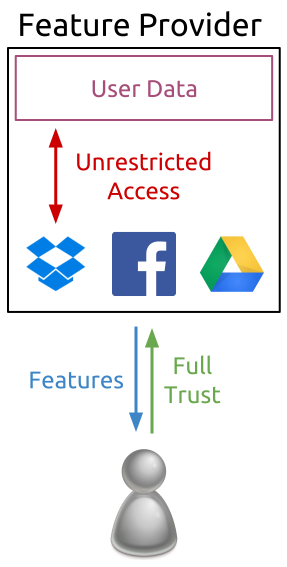
\includegraphics[height=2in]{./figs/out/TrustModel-Traditional.pdf}
    \caption{Traditional Trust Relationship}
    \label{fig:mitigation:trust:traditional}
  \end{subfigure}
  ~
  \begin{subfigure}[t]{0.48\textwidth}
    \centering
    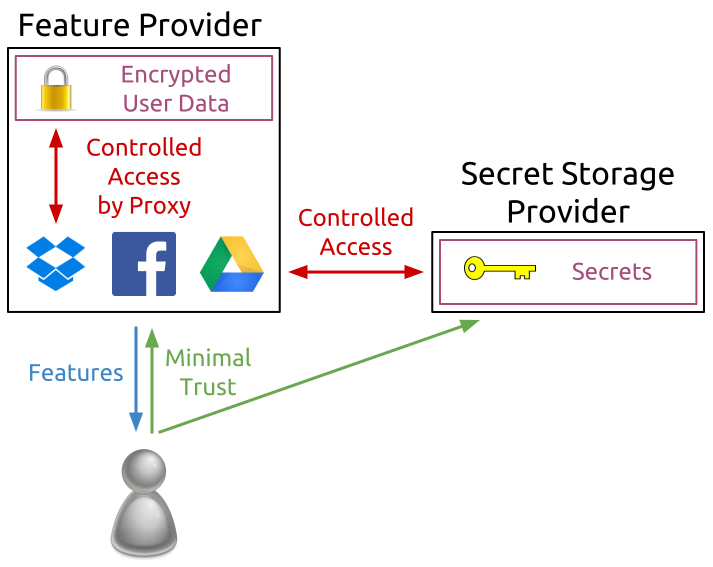
\includegraphics[height=2in]{./figs/out/TrustModel-Seperated.pdf}
    \caption{Distributed Trust Relationship}
    \label{fig:mitigation:trust:distributed}
  \end{subfigure}
  \caption{SSaaS Model Relationships}
  \label{fig:mitigation:trust}
\end{figure}

Techniques such as SSaaS are a form of ``trust distribution'' -- a
technique for reducing trust in individual third parties by instead
spreading it across multiple parties. Similar techniques have been
used within cryptographic protocols for the purpose of eliminating
single-points-of-trust in the past~\cite{shamir1979}.\footnote{Such
  techniques also bear some resemble to previously proposed ``key
  escrow systems'', albeit with a somewhat opposite
  end-goal~\cite{denning1996}: escrow systems aim to allow additional
  third parties access to user data whereas trust distribution systems
  aim to reduce the access to user data any single party can achieve.}
Trust distribution techniques are capable of allowing users to reduce
or eliminate trust surpluses across a range of use cases without
introducing significant additional usage burdens. While there are
approaches to limiting third party trust that aim to avoid trusting
any third party (e.g. the OTR chat protocol~\cite{otr-v3}), such
techniques are often difficult to apply generally or to use without
creating additional usability challenges. Trust distribution
strategies, however, provide a relatively generic framework for
eliminating trust in any single third party.\footnote{When coupled
  with techniques such as~\cite{shamir1979}, trust distribution
  techniques can eliminate trust in even larger subsets of third
  parties, e.g. not having to trust up to three of five total
  parties.}

To summarize, the proposed recipe for reducing the number of trusted
capabilities afforded to third parties is as follows:

\begin{packed_enum}
\item Identity any surplus capabilities
\item Leverage cryptographic techniques to limit third party access to
  these capabilities
\item Leverage trust distribution techniques to store and control
  access to the secrets required by the aforementioned cryptographic
  techniques in a manner that avoids burdening the end user with the
  need to manage such secrets manually.
\end{packed_enum}

This process eliminates trust surpluses by distributing user trust
across multiple third parties so that individual third parties can not
subvert this trust. As mentioned in \S~\ref{sec:analysis:violations},
such arrangements do run the risk of encouraging collusion-type trust
violations where multiple third parties work together to regain
capabilities that have been denied to them individually. Nonetheless,
such collusion violations are strictly less likely to occur than
single-party violations since they require multiple parties to all be
willing to commit an equivalent single-party violation in concert. The
techniques discussed in the next section for disincentivizing
single-party violations thus also help to disincentive collusion
violations.

\subsection{Disincentivizing Violations}
\label{sec:mitigation:violations}

Beyond limiting the number of capabilities users must entrust to third
parties, it is also desirable to disincentivize the mechanisms by
which third parties might violate such trust.  While technological
solutions provide options for reducing the degree of trust, it is
largely policy solutions that will drive the disincentivization of
common classes of trust violations. By disincentivizing certain
classes of trust violations, we can reduce the likelihood that third
parties will commit such violations, leading to more ``trustworthy''
third parties and fewer instances of trust violations. There are a
variety of mechanisms that one might employ with an aim toward
disincentivizing trust violations.

\subsubsection{Distributed Trust Markets}

In today's traditional third party trust relationships, users
primarily select third party services on the basis of their
features. When users pay for these services, they're primarily paying
to support the core features such services provide. Privacy and
security, while potential end user concerns, are at best secondary
goals. Furthermore, on many free cloud services, the ability to
harvest user data is the basis of the service provider's business
model. As discussed in Section~\ref{sec:mitigation:capabilities},
these situations create a number of perverse incentives in terms of a
third party's respect for user security and privacy. In the first
case, the third party simply does not prioritize user security since
that is not the basis on which users are choosing to use a service. In
the second case, a third party actively works to subvert user security
in order to further leverage user data for the generation of profit.

Distributed trust relationships (Figure~\ref{fig:mitigation:trust}),
such as those employed by the aforementioned SSaaS model, aim to
rectify these issues by introducing additional third party actors
whose primary goal is the protection of user secrets and, by proxy,
the data such secrets can be used to cryptographically protect. The
ability of distributed trust architectures to separate
privacy-oriented secret storage duties from feature-oriented service
provider duties allows users to select each service on the basis of
its associated merits. This quality avoids the issues associated with
putting desirable features in direct competition with security and
privacy -- a competition that security and privacy have historically
lost. Distributed trust relationships not only allow users to
eliminate trust surpluses as discussed in
\S~\ref{sec:mitigation:capabilities}, they also allow users to escape
from traditional, but largely artificial, trade-offs between desirable
third party features and the control of their data.

By severing desirable features from desirable security-enhancing
properties, independent markets can form around feature provision and
secret protection, optimized for the respective priorities of each
field. A distributed trust ecosystem is thus able to make security and
privacy tradable commodities, and to leverage market powers to price
and improve both. A competitive market for secret storage has a number
of security and privacy enhancing benefits:

\begin{packed_desc}
\item[Reputation:] A user's ability to easily switch between secret
  storage providers forces providers to compete on the basis of their
  security and privacy preserving reputations.\footnote{In order to
    achieve such mobility, it is likely necessary to standardize a
    common distributed trust protocol~\cite{sayler-phd}.} Providers
  who do a superior job avoiding the trust violations discussed in
  \S~\ref{sec:analysis:violations} can attract more users and/or
  command a higher price for their services. Since a secret storage
  provider's reputation is tied solely to their ability to faithfully
  protect user secrets, they will not be able to ``iron over'' any
  privacy-related reputation failings with superior end user feature
  sets -- a practice employed by many traditional feature
  providers.\footnote{As an example, consider Facebook's numerous
    trust violations~\cite{goel2014, lomas2014, tsukayama2014} and the
    fact that such violations have had no noticeable impact on the
    number of people using Facebook~\cite{foster2014}. A secret
    storage provider would enjoy no such network benefit from
    providing additional services beyond secret storage were they to
    violate user trust; instead, users would simply switch to a new
    provider.}
\item[Multiple Providers:] A healthy ecosystem of competing secret
  storage providers allows users to select from multiple independent
  providers over which they may further distribute their trust beyond
  a binary ``feature provider + secret storage provider''
  relationship. Such secret ``sharding'' provides a number of benefits
  over relying on a single SSP, from additional trust reduction to
  data redundancy.
\item[Cost:] As in other competitive markets, having a number of
  competing providers will allow the user to select a provider that
  offers the best combination of cost and service.
\end{packed_desc}

Distributed trust markets are potentially useful for disincentivizing
a range of trust violations, from implicit violations to unintentional
violations. Such markets help align economic incentives with practices
that do not favor such violations.

\subsubsection{Digital Due Process}

While mechanisms such as distributed trust markets are useful for
disincentivizing the implicit, unintentional, and colluding classes of
trust violations, other mechanisms are needed to disincentivize
compelled violations. While, trust markets potentially encourage third
parties to push back against compelled trust violations to the maximum
extent permitted under the law, they do little to protect users in
cases where the law requires such violations. While there are some
cases where such violations are in the public interest, it appears
that in many (if not most) compelled violation cases, the public
interest is not well served~\cite{greenwald-collect,
  greenwald-prism}. To reduce unnecessary compelled violations, it is
important to ensure ``digital due process'' rights.

The first step toward protecting such rights is to ensure that user
data stored or processed by third party services receives the same
level of protection as data stored or processed locally. This concept
runs counter to the Third Party Doctrine established by current
U.S. case law~\cite{thompson-thirdparty}. This doctrine holds that
individuals who voluntarily store their data with third parties have
no ``reasonable expectation of privacy'' for such
data~\cite{scotus-katzvus}. While this viewpoint may have made sense
in the mid-20\textsuperscript{th} century when it was established by a
series of Supreme Court rulings~\cite{scotus-usvmiller-privacy,
  scotus-smithvmaryland}, it does not translate well to a world where
third party access to user data is the norm. As shown in
\S~\ref{sec:analysis:violations}, compelled violations are a growing
trend, and in many cases such violations are served via third party
doctrine mechanisms. Such trends suggest a likely overreach of
government data collection, leading to a range of adverse ``chilling''
effects (e.g.~\cite{penney2016}). One possible way of halting or
reversing this trend would be to eliminate the third party doctrine
and begin requiring 4\textsuperscript{th} Amendment warrants in order
to compel third parties to provide or modify user data.

Recently, changes to the third party doctrine have begun to progress
on multiple fronts. Recent Supreme Court decisions have suggested a
willingness to expand user privacy rights in the digital realm, and
may eventually lead the Supreme Court to revisit the third party
doctrine directly~\cite{scotus-usvjones}.  Congress has also long
debated updates to third party doctrine-derived laws such the
Electronic Communications Privacy Act (ECPA)~\cite{ecpa} to include a
warrant requirement for digitally stored
emails~\cite{eff-ecpareform}. Recently, the U.S. House of
Representatives unanimously passed a bill amending the ECPA to require
warrants in most cases~\cite{trujillo-ecpa}. These movements suggest
growing recognition of the due process rights of digital data,
regardless of whether it is stored locally or by third parties. Such
trends likely represent the best hope for reducing unnecessary
compelled violations, ensuring such violations only occur in cases
where the public interest is significantly favored by the compelled
violation of user trust.

\subsubsection{Third Party Liability}

Another mechanism for disincentivizing trust violations, especially of
the unintentional variety, would be to establish standards of
liability for trust violations that result in harms to user
privacy. If a third party violates a user's trust and harms the user
in the process, it is reasonable to expect that users should be able
to seek some measure of relief from such violations. Trust violation
liability would follow the growing trend toward holding companies
liable for digital data breaches resulting from poor security
practices (e.g.~\cite{ftc-asus}).

The nature of this liability could take several forms. The most
obvious form would be to impose civil liability commensurate with the
harm caused by a trust violation on the party committing the
violation. This opens up the thorny issue of how to value such
harms. Anecdotally, how much a user is harmed by a trust violation
varies widely from case to case. For example, the harm from a trust
violation resulting in the public exposure of a set of not
particularly sensitive scenic landscape photos is likely to be far
less than that caused by a violation that leaks trade secrets, medical
data, or other sensitive material~\cite{acquisti2013, romanosky2009}.

One way to overcome this challenge would be to have users declare the
value of the harm that would result from the misuse of trust
capabilities when entrusting third parties with such
capabilities. This approach is similar to the manner in which one
might declare the value of a parcel when shipping it for the purpose
of securing insurance. Third parties could even use such declarations
to charge a user varying amounts for the services they provide --
entrusting a third party with access to more ``valuable'' data would
increase the cost of the provided service to the end user, while
entrusting a third party with access to less ``valuable'' data would
reduce the cost. The damages owed to the user in the event that the
third party violates their trust could then be calculated relative to
this value. In cases where a trust violation occurs due to an
unforeseeable event or otherwise through no negligence on the part of
the third party (e.g. a flaw in a respected external code library or
similar unintentional trust violation), the user would be reimbursed
at or below the declared value of the harm. In the case where trust is
violated due to third party negligence, malpractice, or malfeasance,
(e.g. an implicit or particularly egregious unintentional trust
violation) the user would be reimbursed several multiples of the
declared harm (e.g. similar to the statutory damage multiplier
leveraged in some intellectual property cases where the infringement
is found to be ``willful'').

In addition to allowing users to seek compensation for harm suffered
due to third party trust violations, this approach also further
incentivizes the use of distributed trust architectures. Since such
architectures reduce the number of capabilities with which any single
third party must be trusted, they also reduce the declared value of
any associated harms. For example, the loss of user data (violation of
the \emph{S} capability) is in most cases a lessor harm than the
public exposure of user data (violation of the \emph{R}
capability). By distributing trust across multiple parties, the user
devalues the harm each party can inflict, allowing the user to declare
lower harm costs and pay less for the third party services they use. A
mechanism of trust-violation liability both incentivizes users to
spread their trust across multiple parties and encourages third
parties to avoid any trust violation that would require them to pay
out the associated damages.

To manage this liability, third parties would likely be required to
secure insurance to cover the cost of damages in the event that a
trust violation occurs~\cite{ciab2015, starks2016}.\footnote{It is
  even possible that the government itself might act as such an
  insurer (or insurance underwriter), as they currently do with banks
  via the Federal Deposit Insurance Corporation (FDIC)~\cite{fdic}.}
These insurers would be in a position to provide additional economic
disincentives to third party trust violations. For example, insurers
could charge each third party on the basis of how ``secure'' (or the
inverse, how ``risky'') a third party's infrastructure is. Third
parties who employ additional security protections or who otherwise
adhere to security best practices would end up paying lower insurance
premiums to indemnify them against claims for trust violation damages.

Regardless of mechanism, establishing a standard system for trust
violation liability will help disincentivize trust violations via a
variety of mechanisms. Tying financial penalties to such undesirable
behaviors encourages third parties to avoid trust violations, even
when such parties act only in their own self interest. Using a
declaratory harm valuation model avoids the challenges associated with
properly accessing the harm caused by breaches of user privacy, and
provides a straightforward mechanism for compensating users for
breaches of third party trust.

%%  LocalWords:  SSaaS SSP OTR FP th ECPA

\section{Conclusion}
\label{sec:conclusion}

The pervasiveness of third parties across the modern cloud computing
landscape is undeniable. What this pervasiveness means for the privacy
and security of users and their data is an area of active research. In
this paper, I presented a biaxial model for evaluating third party
trust by both degree of trust and manner of violation. I then applied
this model to a variety of popular third party services as well as
examples of historic trust violations. This analysis is useful in
helping to understand the manners in which user privacy relies on
trusted third parties as well as the motivations that might undercut
this trust. Finally, I provided a number of suggestions for reducing
both the degree of third party trust (e.g. via the use of distributed
trust architectures) as well as for disincentivizing common classes of
trust violations. While these techniques are unlikely to eliminate the
privacy and security risks inherent to the use of trusted third
parties, I hope they provide a basis on which such risks can begin to
be measured and reduced.


\clearpage
\bibliographystyle{acm}
\bibliography{refs}

\end{document}
